Many recent international roadmaps for computer systems research
appeal to reinvent computing~\cite{hipeac_roadmap2017,Dongarra:2011:IES:1943326.1943339,prace}.
%
Indeed, developing, benchmarking, optimizing and co-designing hardware and software
has never been harder, no matter if it is for embedded and IoT devices,
or data centers and Exascale supercomputers.
%
This is caused by both physical limitations of existing technologies
and an unmanageable complexity of continuously changing computer systems
which already have too many design and optimization choices and objectives
to consider at all software and hardware levels~\cite{fursin:hal-01054763},
as conceptually shown in Figure~\ref{fig:introduction}.
%
That is why most of these roadmaps now agree with our vision
that such problems should be solved in a close collaboration
between industry, academia and end-users~\cite{Fur2009,cm:29db2248aba45e59:cd11e3a188574d80}.

   %%%%%%%%%%%%%%%%%%%%%%%%%%%%%%%%%%%%%%%%%%%%%%%%%%%%%%%%%%%%%%%%%%%%%%%%%%%%%%%%%%%%%%%%%
   %CK={"action":"prepare_for_latex", "cid":"slide:0ab24e3fa8acab0a", "file":"d6118462b94f89da-cropped.pdf", "path":"ck-assets", "ck_image":"yes", "ck_image_width":600}

   \begin{figure*}[htb]
     \centering
      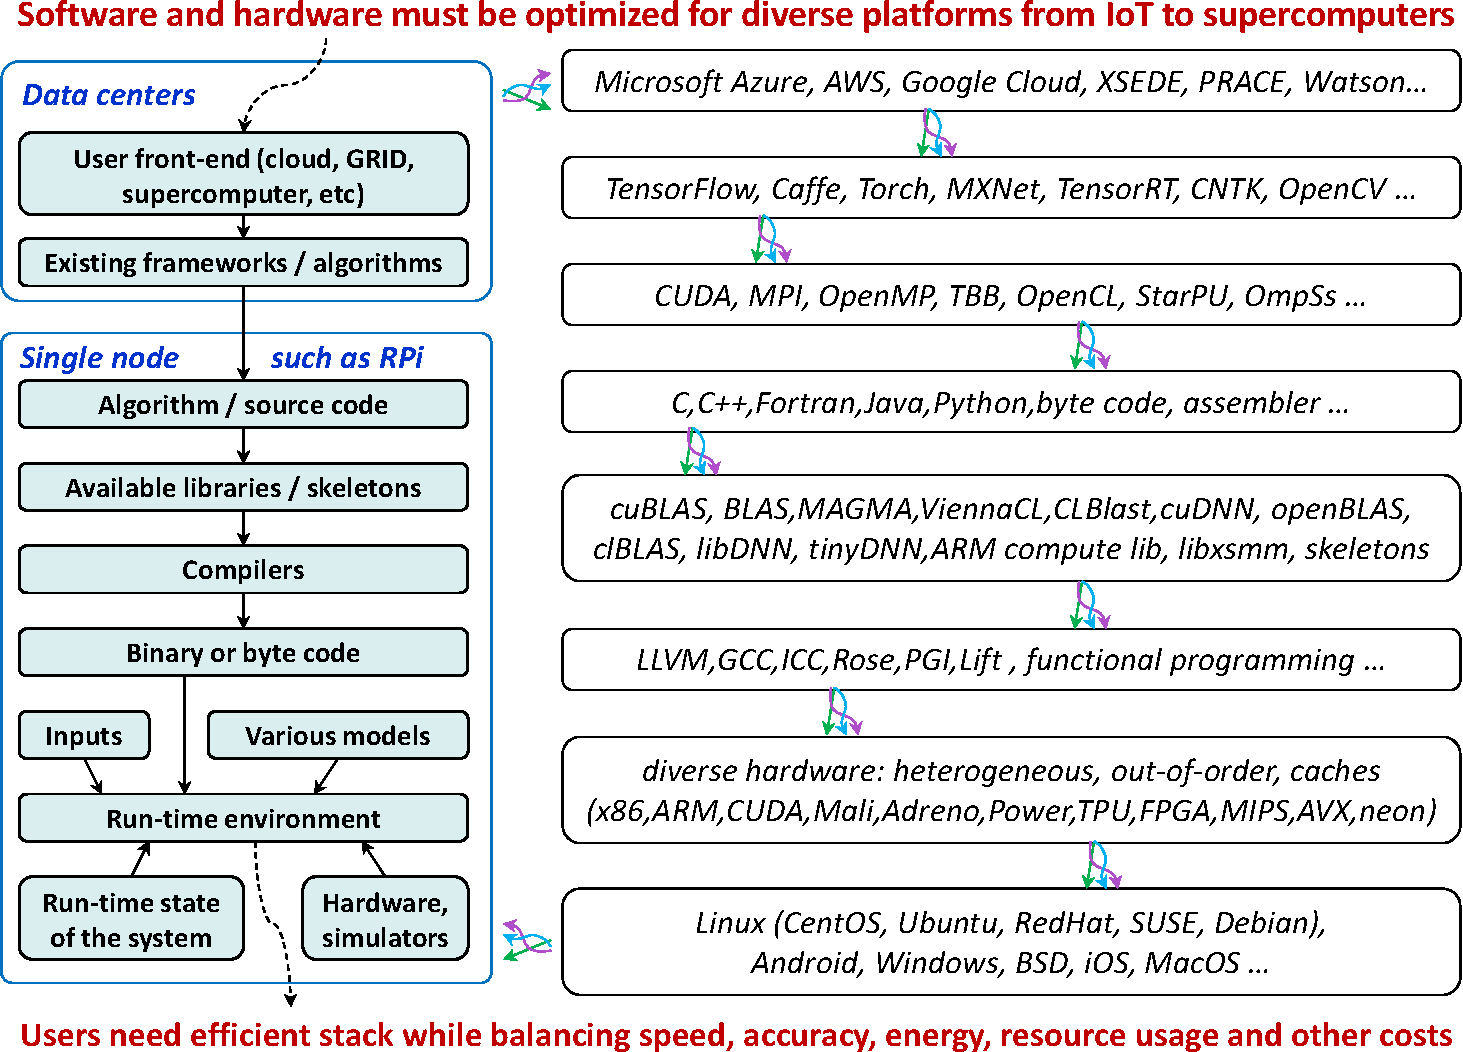
\includegraphics[width=5.2in]
      {ck-assets/d6118462b94f89da-cropped.pdf} %CK_URL={d6118462b94f89da-cropped.pdf}

     \caption{
       Too many design and optimization choices at all levels of the continuously changing software and hardware stack
       make it extremely challenging and time consuming to design efficient computer systems for realistic workloads.
     }

     \label{fig:introduction}
   \end{figure*}
   %%%%%%%%%%%%%%%%%%%%%%%%%%%%%%%%%%%%%%%%%%%%%%%%%%%%%%%%%%%%%%%%%%%%%%%%%%%%%%%%%%%%%%%%%

However, after we initiated artifact evaluation (AE)~\cite{ctuning-ae1,childers2016artifact}
at several premier ACM and IEEE conferences to reproduce and validate experimental results 
from published papers, we noticed an even more
fundamental problem: a growing technology transfer gap between academic
research and industrial development.
%
After evaluating more than 100 artifacts from the leading computer systems conferences
in the past 4 years, we noticed that only a small fraction of research artifacts 
could be easily customized, ported to other environments and hardware, reused, 
and built upon.
%
We have grown to believe that this due to a lack of a common workflow framework
that could simplify implementation and sharing of artifacts and workflows as
portable, customizable and reusable components with some common API and meta information
vital for open science~\cite{new_pub_model}.

At the same time, companies are always under pressure and rarely have time to
dig into numerous academic artifacts shared as CSV/Excel files
and ``black box'' VM and Docker images, or adapt numerous ad-hoc scripts 
to realistic and ever changing workloads, software and hardware.
%
That is why promising techniques may remain in academia for decades while just
being incrementally improved, put on the shelf when leading students graduate,
and ``reinvented'' from time to time.

Autotuning is one such example: this very popular technique has been actively
researched since the 1990s to automatically explore large optimization spaces
and improve efficiency of computer systems~\cite{atlas, fftw, CSS99, VE00,
FOK02, Tapus:2002:AHT:762761.762771, vista, spiral, LCYP04, la2004, PE2006,
Shende:2006:TPP:1125980.1125982, 1742-6596-125-1-012089,
DBLP:conf/ipps/HartonoNS09, 29db2248aba45e59:a31e374796869125, tnld10,
openbenchmarking, Ren:2010:GPC:1849301.1849332, Grauer-Gray2012-hn,
DBLP:conf/cgo/GreweWO13, Khan:2013:SAC:2400682.2400690, ansel:pact:2014,
DBLP:conf/sc/TsaiLKD16, DBLP:conf/supercomputer/AbdelfattahHTD16}.
%
Every year, dozens of autotuning papers get published to optimize some computer
system components, improve and speed up exploration and co-design strategies,
and enable run-time adaptation.
%
Yet, when trying to make autotuning practical (in particular, by applying
machine learning) we faced numerous challenges with integrating such published
techniques into real, complex and continuously evolving software and hardware
stack~\cite{Fur2009,fursin:hal-01054763,cm:29db2248aba45e59:cd11e3a188574d80,new_pub_model}.

Eventually, these problems motivated us to develop a common experimental
framework and methodology similar to physics and other natural sciences to
collaboratively improve autotuning and other techniques.
%
As part of this educational initiative, we implemented an extensible, portable
and technology-agnostic workflow for autotuning using the open-source
Collective Knowledge framework (CK)~\cite{ck,ck-date16}.
%
Such workflows help researchers to reuse already shared applications, kernels,
data sets and tools, or add their own ones using a common JSON API and
meta-description~\cite{json-org}. 
%
Moreover, such workflows can automatically
adapt compilation and execution to a given environment on a given device
using integrated cross-platform package manager.

Our approach takes advantage of a powerful and holistic top-down methodology
successfully used in physics and other sciences when learning complex systems.
%
The key idea is to let novice researchers first master simple compiler flag
autotuning scenarios while learning interdisciplinary techniques including
machine learning and statistical analysis.
%
Researchers can then gradually increase complexity to enable automatic and
collaborative co-design of the whole SW/HW stack by exposing more design and
optimization choices, multiple optimization objectives (execution time, code
size, power consumption, memory usage, platform cost, accuracy, etc.),
crowdsource autotuning across diverse devices provided by volunteers similar to
SETI@home~\cite{Anderson:2002:SEP:581571.581573}, 
continuously exchange and discuss optimization results, and
eventually build upon each other's results.

We use our approach to optimize diverse kernels and real workloads such as {\tt
zlib} in terms of speed and code size by crowdsourcing compiler flag autotuning
across Raspberry Pi3 devices using the default GCC 4.9.2 and the latest GCC
7.1.0 compilers.
%
We have been able to achieve up to 50\% reductions in code size and from 15\%
to 8 times speed ups across different workloads over the ``-O3'' baseline.
%
Our CK workflow and all related artifacts are available at GitHub 
to allow researchers to compare and improve various exploration strategies 
(particularly based on machine learning algorithms such as KNN, GA, SVM,
deep learning, though further documentation of APIs is still 
required)~\cite{29db2248aba45e59:a31e374796869125,cm:29db2248aba45e59:cd11e3a188574d80}.
%
We have also shared all experimental results in our open repository of
optimization knowledge~\cite{live-ck-repo,live-ck-repo-rpi-gcc710} to be
validated and reproduced by the community.

We hope that our approach will serve as a practical foundation
for open, reproducible and sustainable computer systems research
by connecting students, scientists, end-users, hardware designers
and software developers to learn together how to co-design
next generation of efficient and self-optimizing computer systems,
particularly via reproducible competitions such as ReQuEST~\cite{request}.
%

This technical report is organized as follows.
%
Section~\ref{sec:converting} introduces the Collective Knowledge framework (CK)
and the concept of sharing artifacts as portable, customizable and reusable components.
%
Section~\ref{sec:autotuning} describes how to implement a customizable,
multi-dimensional and multi-objective autotuning as a CK workflow.
%
Section~\ref{sec:flag_autotuning} shows how to optimize compiler flags using
our universal CK autotuner.
%
Section~\ref{sec:crowdtuning} presents a snapshot of the latest optimization
results from collaborative tuning of GCC flags for numerous shared workloads
across Raspberry Pi3 devices.
%
Section~\ref{sec:collaborative} shows optimization results of zlib and other
realistic workloads for GCC 4.9.2 and GCC 7.1.0 across Raspberry Pi3 devices.
%
Section~\ref{sec:crowdfuzzing} describes how implement and crowdsource fuzzing
of compilers and systems for various bugs using our customizable CK autotuning workflow.
%
Section~\ref{sec:crowdmodeling} shows how to predict optimizations via CK for previously
unseen programs using machine learning.
%
Section~\ref{sec:features} demonstrates how to select and autotune models
and features to improve optimization predictions while reducing complexity.
%
Section~\ref{sec:datasets} shows how to enable efficient, input-aware and adaptive 
libraries and programs via CK.
%
Section~\ref{sec:competitions} presents CK as an open platform to 
support reproducible and Pareto-efficient co-design competitions 
of the whole software/hardware/model stack for emerging workloads 
such as deep learning and quantum computing.
%
We present future work in Section~\ref{sec:conclusions}.
%
We also included Artifact Appendix to allow students try our framework, 
participate in collaborative autotuning, gradually document APIs and
improve experimental workflows.
